\documentclass[twoside]{book}

% Packages required by doxygen
\usepackage{fixltx2e}
\usepackage{calc}
\usepackage{doxygen}
\usepackage[export]{adjustbox} % also loads graphicx
\usepackage{graphicx}
\usepackage[utf8]{inputenc}
\usepackage{makeidx}
\usepackage{multicol}
\usepackage{multirow}
\PassOptionsToPackage{warn}{textcomp}
\usepackage{textcomp}
\usepackage[nointegrals]{wasysym}
\usepackage[table]{xcolor}

% Font selection
\usepackage[T1]{fontenc}
\usepackage[scaled=.90]{helvet}
\usepackage{courier}
\usepackage{amssymb}
\usepackage{sectsty}
\renewcommand{\familydefault}{\sfdefault}
\allsectionsfont{%
  \fontseries{bc}\selectfont%
  \color{darkgray}%
}
\renewcommand{\DoxyLabelFont}{%
  \fontseries{bc}\selectfont%
  \color{darkgray}%
}
\newcommand{\+}{\discretionary{\mbox{\scriptsize$\hookleftarrow$}}{}{}}

% Page & text layout
\usepackage{geometry}
\geometry{%
  a4paper,%
  top=2.5cm,%
  bottom=2.5cm,%
  left=2.5cm,%
  right=2.5cm%
}
\tolerance=750
\hfuzz=15pt
\hbadness=750
\setlength{\emergencystretch}{15pt}
\setlength{\parindent}{0cm}
\setlength{\parskip}{3ex plus 2ex minus 2ex}
\makeatletter
\renewcommand{\paragraph}{%
  \@startsection{paragraph}{4}{0ex}{-1.0ex}{1.0ex}{%
    \normalfont\normalsize\bfseries\SS@parafont%
  }%
}
\renewcommand{\subparagraph}{%
  \@startsection{subparagraph}{5}{0ex}{-1.0ex}{1.0ex}{%
    \normalfont\normalsize\bfseries\SS@subparafont%
  }%
}
\makeatother

% Headers & footers
\usepackage{fancyhdr}
\pagestyle{fancyplain}
\fancyhead[LE]{\fancyplain{}{\bfseries\thepage}}
\fancyhead[CE]{\fancyplain{}{}}
\fancyhead[RE]{\fancyplain{}{\bfseries\leftmark}}
\fancyhead[LO]{\fancyplain{}{\bfseries\rightmark}}
\fancyhead[CO]{\fancyplain{}{}}
\fancyhead[RO]{\fancyplain{}{\bfseries\thepage}}
\fancyfoot[LE]{\fancyplain{}{}}
\fancyfoot[CE]{\fancyplain{}{}}
\fancyfoot[RE]{\fancyplain{}{\bfseries\scriptsize Generated by Doxygen }}
\fancyfoot[LO]{\fancyplain{}{\bfseries\scriptsize Generated by Doxygen }}
\fancyfoot[CO]{\fancyplain{}{}}
\fancyfoot[RO]{\fancyplain{}{}}
\renewcommand{\footrulewidth}{0.4pt}
\renewcommand{\chaptermark}[1]{%
  \markboth{#1}{}%
}
\renewcommand{\sectionmark}[1]{%
  \markright{\thesection\ #1}%
}

% Indices & bibliography
\usepackage{natbib}
\usepackage[titles]{tocloft}
\setcounter{tocdepth}{3}
\setcounter{secnumdepth}{5}
\makeindex

% Hyperlinks (required, but should be loaded last)
\usepackage{ifpdf}
\ifpdf
  \usepackage[pdftex,pagebackref=true]{hyperref}
\else
  \usepackage[ps2pdf,pagebackref=true]{hyperref}
\fi
\hypersetup{%
  colorlinks=true,%
  linkcolor=blue,%
  citecolor=blue,%
  unicode%
}

% Custom commands
\newcommand{\clearemptydoublepage}{%
  \newpage{\pagestyle{empty}\cleardoublepage}%
}

\usepackage{caption}
\captionsetup{labelsep=space,justification=centering,font={bf},singlelinecheck=off,skip=4pt,position=top}

%===== C O N T E N T S =====

\begin{document}

% Titlepage & ToC
\hypersetup{pageanchor=false,
             bookmarksnumbered=true,
             pdfencoding=unicode
            }
\pagenumbering{roman}
\begin{titlepage}
\vspace*{7cm}
\begin{center}%
{\Large Lexer }\\
\vspace*{1cm}
{\large Generated by Doxygen 1.8.11}\\
\end{center}
\end{titlepage}
\clearemptydoublepage
\tableofcontents
\clearemptydoublepage
\pagenumbering{arabic}
\hypersetup{pageanchor=true}

%--- Begin generated contents ---
\chapter{Lexer}
\label{md_README}
\hypertarget{md_README}{}
\subsection*{Description}

This is a repository containing my implementation of a lexer, based on the following lecture\+: \href{http://hjemmesider.diku.dk/~torbenm/Basics/basics_lulu2.pdf}{\tt Basics of Compiler Design}

\subsection*{Todo}

\mbox{[}x\mbox{]} \hyperlink{classNFA}{N\+FA} to D\+FA transformation \mbox{[}x\mbox{]} Detecting tokens \mbox{[}x\mbox{]} File loading \mbox{[}x\mbox{]} File saving \mbox{[} \mbox{]} Write documentation \mbox{[} \mbox{]} Report lexical errors instead of terminating the program \mbox{[} \mbox{]} Use a better structure to represent token types \mbox{[} \mbox{]} Add more infos to the tokens payload \mbox{[} \mbox{]} Clean the code \mbox{[} \mbox{]} (Not really related) Write the complete set of tokens for the test language \mbox{[} \mbox{]} Graph optimization 
\chapter{Hierarchical Index}
\doxysection{Class Hierarchy}
This inheritance list is sorted roughly, but not completely, alphabetically\+:\begin{DoxyCompactList}
\item \contentsline{section}{Lexer}{\pageref{classLexer}}{}
\item \contentsline{section}{N\+FA}{\pageref{classNFA}}{}
\item \contentsline{section}{N\+F\+A\+IO}{\pageref{classNFAIO}}{}
\item runtime\+\_\+error\begin{DoxyCompactList}
\item \contentsline{section}{Lexical\+Error\+Exception}{\pageref{classLexicalErrorException}}{}
\end{DoxyCompactList}
\item \contentsline{section}{State}{\pageref{structState}}{}
\item \contentsline{section}{Token\+Info}{\pageref{structTokenInfo}}{}
\item \contentsline{section}{Traverser}{\pageref{classTraverser}}{}
\end{DoxyCompactList}

\chapter{Class Index}
\section{Class List}
Here are the classes, structs, unions and interfaces with brief descriptions\+:\begin{DoxyCompactList}
\item\contentsline{section}{\hyperlink{classLexer}{Lexer} }{\pageref{classLexer}}{}
\item\contentsline{section}{\hyperlink{classLexicalErrorException}{Lexical\+Error\+Exception} }{\pageref{classLexicalErrorException}}{}
\item\contentsline{section}{\hyperlink{classNFA}{N\+FA} }{\pageref{classNFA}}{}
\item\contentsline{section}{\hyperlink{classNFAIO}{N\+F\+A\+IO} }{\pageref{classNFAIO}}{}
\item\contentsline{section}{\hyperlink{structState}{State} }{\pageref{structState}}{}
\item\contentsline{section}{\hyperlink{structTokenInfo}{Token\+Info} }{\pageref{structTokenInfo}}{}
\item\contentsline{section}{\hyperlink{classTraverser}{Traverser} }{\pageref{classTraverser}}{}
\end{DoxyCompactList}

\chapter{Class Documentation}
\hypertarget{classLexer}{}\section{Lexer Class Reference}
\label{classLexer}\index{Lexer@{Lexer}}


{\ttfamily \#include $<$Lexer.\+hpp$>$}

\subsection*{Public Member Functions}
\begin{DoxyCompactItemize}
\item 
\hyperlink{classLexer_adbbd9373db0da3c2a5529e382d682cb2}{Lexer} (const \hyperlink{classNFA}{N\+FA} \&nfa)
\item 
std\+::vector$<$ std\+::pair$<$ std\+::string, std\+::string $>$ $>$ \hyperlink{classLexer_a631154ac348ea4db3e3a06992fa6245a}{extract\+Tokens} (const std\+::string \&input)
\item 
std\+::pair$<$ bool, std\+::pair$<$ std\+::string, std\+::string $>$ $>$ \hyperlink{classLexer_afd24d0694acffafff7f705cefe2ece21}{next} (const std\+::string \&stream)
\end{DoxyCompactItemize}


\subsection{Detailed Description}
A lexer class. Represent a lexer. 

\subsection{Constructor \& Destructor Documentation}
\index{Lexer@{Lexer}!Lexer@{Lexer}}
\index{Lexer@{Lexer}!Lexer@{Lexer}}
\subsubsection[{\texorpdfstring{Lexer(const N\+F\+A \&nfa)}{Lexer(const NFA &nfa)}}]{\setlength{\rightskip}{0pt plus 5cm}Lexer\+::\+Lexer (
\begin{DoxyParamCaption}
\item[{const {\bf N\+FA} \&}]{nfa}
\end{DoxyParamCaption}
)}\hypertarget{classLexer_adbbd9373db0da3c2a5529e382d682cb2}{}\label{classLexer_adbbd9373db0da3c2a5529e382d682cb2}
A constructor. Constructs a lexer from a \hyperlink{classNFA}{N\+FA} representing the detected lexic. 

\subsection{Member Function Documentation}
\index{Lexer@{Lexer}!extract\+Tokens@{extract\+Tokens}}
\index{extract\+Tokens@{extract\+Tokens}!Lexer@{Lexer}}
\subsubsection[{\texorpdfstring{extract\+Tokens(const std\+::string \&input)}{extractTokens(const std::string &input)}}]{\setlength{\rightskip}{0pt plus 5cm}std\+::vector$<$ std\+::pair$<$ std\+::string, std\+::string $>$ $>$ Lexer\+::extract\+Tokens (
\begin{DoxyParamCaption}
\item[{const std\+::string \&}]{input}
\end{DoxyParamCaption}
)}\hypertarget{classLexer_a631154ac348ea4db3e3a06992fa6245a}{}\label{classLexer_a631154ac348ea4db3e3a06992fa6245a}
A function that extracts token from the given input and returns a list of tokens. 
\begin{DoxyParams}{Parameters}
{\em input} & a std\+::string representing the input text \\
\hline
\end{DoxyParams}
\index{Lexer@{Lexer}!next@{next}}
\index{next@{next}!Lexer@{Lexer}}
\subsubsection[{\texorpdfstring{next(const std\+::string \&stream)}{next(const std::string &stream)}}]{\setlength{\rightskip}{0pt plus 5cm}std\+::pair$<$ bool, std\+::pair$<$ std\+::string, std\+::string $>$ $>$ Lexer\+::next (
\begin{DoxyParamCaption}
\item[{const std\+::string \&}]{stream}
\end{DoxyParamCaption}
)}\hypertarget{classLexer_afd24d0694acffafff7f705cefe2ece21}{}\label{classLexer_afd24d0694acffafff7f705cefe2ece21}
A function that extracts the next token from the input. 
\begin{DoxyParams}{Parameters}
{\em stream} & a std\+::string representing the input text \\
\hline
\end{DoxyParams}


The documentation for this class was generated from the following files\+:\begin{DoxyCompactItemize}
\item 
include/Lexer.\+hpp\item 
src/Lexer.\+cpp\end{DoxyCompactItemize}

\hypertarget{classLexicalErrorException}{}\doxysection{Lexical\+Error\+Exception Class Reference}
\label{classLexicalErrorException}\index{LexicalErrorException@{LexicalErrorException}}


{\ttfamily \#include $<$Lexical\+Error\+Exception.\+hpp$>$}

Inheritance diagram for Lexical\+Error\+Exception\+:\begin{figure}[H]
\begin{center}
\leavevmode
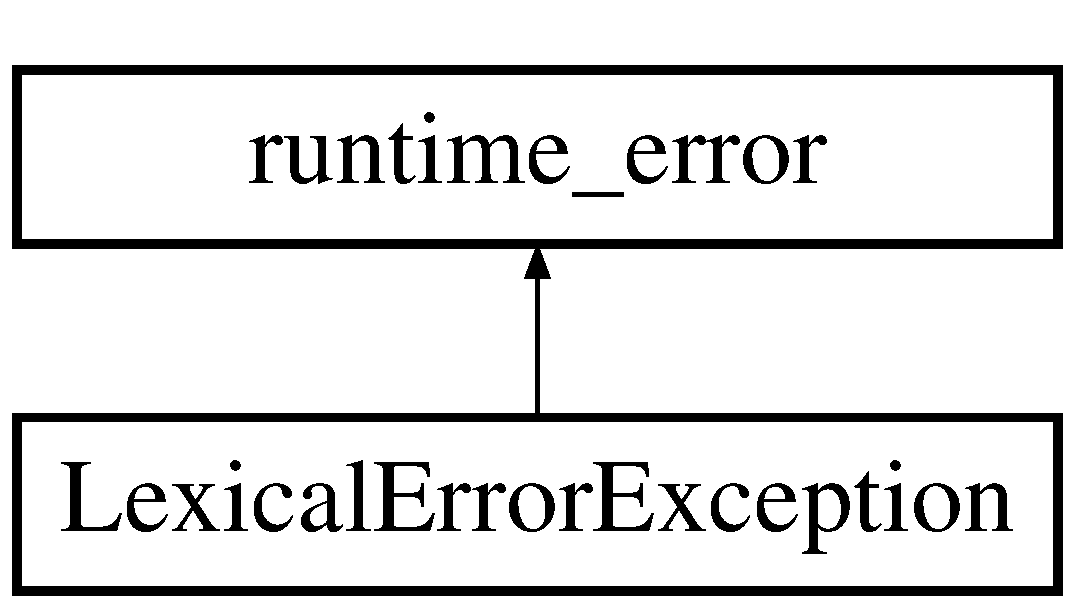
\includegraphics[height=2.000000cm]{classLexicalErrorException}
\end{center}
\end{figure}
\doxysubsection*{Public Member Functions}
\begin{DoxyCompactItemize}
\item 
\mbox{\hyperlink{classLexicalErrorException_a9ccea8291962d41fd6e215e6460e0bd0}{Lexical\+Error\+Exception}} (const std\+::string \&msg=\char`\"{}\char`\"{})
\end{DoxyCompactItemize}


\doxysubsection{Detailed Description}
An exception class. Thrown when a lexical error has been detected. 

\doxysubsection{Constructor \& Destructor Documentation}
\mbox{\Hypertarget{classLexicalErrorException_a9ccea8291962d41fd6e215e6460e0bd0}\label{classLexicalErrorException_a9ccea8291962d41fd6e215e6460e0bd0}} 
\index{LexicalErrorException@{LexicalErrorException}!LexicalErrorException@{LexicalErrorException}}
\index{LexicalErrorException@{LexicalErrorException}!LexicalErrorException@{LexicalErrorException}}
\doxysubsubsection{\texorpdfstring{LexicalErrorException()}{LexicalErrorException()}}
{\footnotesize\ttfamily Lexical\+Error\+Exception\+::\+Lexical\+Error\+Exception (\begin{DoxyParamCaption}\item[{const std\+::string \&}]{msg = {\ttfamily \char`\"{}\char`\"{}} }\end{DoxyParamCaption})}

A constructor. Constructs the error with the given message. 

The documentation for this class was generated from the following files\+:\begin{DoxyCompactItemize}
\item 
include/Lexical\+Error\+Exception.\+hpp\item 
src/Lexical\+Error\+Exception.\+cpp\end{DoxyCompactItemize}

\hypertarget{classNFA}{}\section{N\+FA Class Reference}
\label{classNFA}\index{N\+FA@{N\+FA}}
\subsection*{Public Member Functions}
\begin{DoxyCompactItemize}
\item 
{\bfseries N\+FA} (const Alphabet \&alphabet)\hypertarget{classNFA_ae8841f4b0dbe122187e2a64c73643769}{}\label{classNFA_ae8841f4b0dbe122187e2a64c73643769}

\item 
{\bfseries N\+FA} (const Alphabet \&alphabet, const std\+::vector$<$ \hyperlink{structState}{State} $>$ \&states, const std\+::map$<$ std\+::pair$<$ size\+\_\+t, Char\+Type $>$, size\+\_\+t $>$ \&character\+Transition\+Table, const std\+::map$<$ size\+\_\+t, std\+::vector$<$ size\+\_\+t $>$$>$ \&empty\+Transition\+Table=std\+::map$<$ size\+\_\+t, std\+::vector$<$ size\+\_\+t $>$$>$())\hypertarget{classNFA_ae7fe25f259e31506f1358608f44b3d24}{}\label{classNFA_ae7fe25f259e31506f1358608f44b3d24}

\item 
{\bfseries N\+FA} (const \hyperlink{classNFA}{N\+FA} \&other)=default\hypertarget{classNFA_ae7303013f54a9f08704ae9b805c38650}{}\label{classNFA_ae7303013f54a9f08704ae9b805c38650}

\item 
{\bfseries N\+FA} (\hyperlink{classNFA}{N\+FA} \&\&other)=default\hypertarget{classNFA_a4d1844d6d9d20506be1d80dd6e81d011}{}\label{classNFA_a4d1844d6d9d20506be1d80dd6e81d011}

\item 
\hyperlink{classNFA}{N\+FA} \& {\bfseries operator=} (const \hyperlink{classNFA}{N\+FA} \&other)=default\hypertarget{classNFA_afad27066b284b7bf217df99a415d292d}{}\label{classNFA_afad27066b284b7bf217df99a415d292d}

\item 
\hyperlink{classNFA}{N\+FA} \& {\bfseries operator=} (\hyperlink{classNFA}{N\+FA} \&\&other)=default\hypertarget{classNFA_aa8a9cfe181878d1ee0279feeab1d46c5}{}\label{classNFA_aa8a9cfe181878d1ee0279feeab1d46c5}

\item 
void {\bfseries add\+State} (const \hyperlink{structState}{State} \&state)\hypertarget{classNFA_a12aa5a3267473c67ad7c75f9d13f2157}{}\label{classNFA_a12aa5a3267473c67ad7c75f9d13f2157}

\item 
void {\bfseries add\+State} (\hyperlink{structState}{State} \&\&state)\hypertarget{classNFA_a01d23e3617878eede7d7e162fa29a990}{}\label{classNFA_a01d23e3617878eede7d7e162fa29a990}

\item 
void {\bfseries add\+Transition} (const \hyperlink{structState}{State} \&from, const Char\+Type \&character, const \hyperlink{structState}{State} \&to)\hypertarget{classNFA_aa1be789eb438068c1297f81cebde3986}{}\label{classNFA_aa1be789eb438068c1297f81cebde3986}

\item 
void {\bfseries add\+Transition} (const \hyperlink{structState}{State} \&from, const \hyperlink{structState}{State} \&to)\hypertarget{classNFA_a8a806166448f5228f1cea02fb3c407e1}{}\label{classNFA_a8a806166448f5228f1cea02fb3c407e1}

\item 
void {\bfseries add\+Transitions} (const \hyperlink{structState}{State} \&from, const Alphabet \&characters, const \hyperlink{structState}{State} \&to)\hypertarget{classNFA_a84585fb96d8fbd4fa978f22389e22f12}{}\label{classNFA_a84585fb96d8fbd4fa978f22389e22f12}

\item 
void {\bfseries add\+Transition} (const std\+::string \&from, const Char\+Type \&character, const std\+::string \&to)\hypertarget{classNFA_a42e23c1d2b811f41410e77c3e3f1f97c}{}\label{classNFA_a42e23c1d2b811f41410e77c3e3f1f97c}

\item 
void {\bfseries add\+Transition} (const std\+::string \&from, const std\+::string \&to)\hypertarget{classNFA_abac152eeed3df6612b6a7ce30d3dc796}{}\label{classNFA_abac152eeed3df6612b6a7ce30d3dc796}

\item 
void {\bfseries add\+Transitions} (const std\+::string \&from, const Alphabet \&characters, const std\+::string \&to)\hypertarget{classNFA_ae81e75d4f68ca63090bf6eeb49f3f833}{}\label{classNFA_ae81e75d4f68ca63090bf6eeb49f3f833}

\item 
void {\bfseries print\+Debug} () const \hypertarget{classNFA_a53ad6f0fa9646d8ffab9427677833164}{}\label{classNFA_a53ad6f0fa9646d8ffab9427677833164}

\item 
\hyperlink{classNFA}{N\+FA} {\bfseries to\+D\+FA} () const \hypertarget{classNFA_ac6fde2f66abcaf39119e5e4ac86056eb}{}\label{classNFA_ac6fde2f66abcaf39119e5e4ac86056eb}

\end{DoxyCompactItemize}
\subsection*{Static Public Member Functions}
\begin{DoxyCompactItemize}
\item 
static \hyperlink{classNFA}{N\+FA} \hyperlink{classNFA_a4ac23a73cb85dbff43bbcf2873dd4f9b}{combine} (const std\+::vector$<$ \hyperlink{classNFA}{N\+FA} $>$ \&nfas)
\begin{DoxyCompactList}\small\item\em Combine multiple \hyperlink{classNFA}{N\+FA} to a single \hyperlink{classNFA}{N\+FA}. \end{DoxyCompactList}\end{DoxyCompactItemize}
\subsection*{Friends}
\begin{DoxyCompactItemize}
\item 
class {\bfseries Traverser}\hypertarget{classNFA_a4ed369a6ee2b54f1b68897a0e9c859a2}{}\label{classNFA_a4ed369a6ee2b54f1b68897a0e9c859a2}

\item 
class {\bfseries N\+F\+A\+IO}\hypertarget{classNFA_a63eedf3dea9b1923c2f1d7e49bd0593b}{}\label{classNFA_a63eedf3dea9b1923c2f1d7e49bd0593b}

\end{DoxyCompactItemize}


\subsection{Member Function Documentation}
\index{N\+FA@{N\+FA}!combine@{combine}}
\index{combine@{combine}!N\+FA@{N\+FA}}
\subsubsection[{\texorpdfstring{combine(const std\+::vector$<$ N\+F\+A $>$ \&nfas)}{combine(const std::vector< NFA > &nfas)}}]{\setlength{\rightskip}{0pt plus 5cm}{\bf N\+FA} N\+F\+A\+::combine (
\begin{DoxyParamCaption}
\item[{const std\+::vector$<$ {\bf N\+FA} $>$ \&}]{nfas}
\end{DoxyParamCaption}
)\hspace{0.3cm}{\ttfamily [static]}}\hypertarget{classNFA_a4ac23a73cb85dbff43bbcf2873dd4f9b}{}\label{classNFA_a4ac23a73cb85dbff43bbcf2873dd4f9b}


Combine multiple \hyperlink{classNFA}{N\+FA} to a single \hyperlink{classNFA}{N\+FA}. 


\begin{DoxyParams}{Parameters}
{\em nfas} & the list of \hyperlink{classNFA}{N\+FA} we want to combine \\
\hline
\end{DoxyParams}
\begin{DoxyReturn}{Returns}
the resulting \hyperlink{classNFA}{N\+FA} 
\end{DoxyReturn}


The documentation for this class was generated from the following files\+:\begin{DoxyCompactItemize}
\item 
include/N\+F\+A.\+hpp\item 
src/N\+F\+A.\+cpp\end{DoxyCompactItemize}

\hypertarget{classNFAIO}{}\section{N\+F\+A\+IO Class Reference}
\label{classNFAIO}\index{N\+F\+A\+IO@{N\+F\+A\+IO}}


{\ttfamily \#include $<$N\+F\+A\+I\+O.\+hpp$>$}

\subsection*{Static Public Member Functions}
\begin{DoxyCompactItemize}
\item 
static \hyperlink{classNFA}{N\+FA} \hyperlink{classNFAIO_a06e1cedc984bdd40daef8e3d5fd2f54d}{load\+From\+Filename} (const std\+::string \&filename)
\item 
static bool \hyperlink{classNFAIO_a17b2b008419263c873e3c46ffaaf7902}{save\+To\+File} (const \hyperlink{classNFA}{N\+FA} \&nfa, const std\+::string \&filename)
\end{DoxyCompactItemize}


\subsection{Detailed Description}
A helper class. Used to read/write lexics. 

\subsection{Member Function Documentation}
\index{N\+F\+A\+IO@{N\+F\+A\+IO}!load\+From\+Filename@{load\+From\+Filename}}
\index{load\+From\+Filename@{load\+From\+Filename}!N\+F\+A\+IO@{N\+F\+A\+IO}}
\subsubsection[{\texorpdfstring{load\+From\+Filename(const std\+::string \&filename)}{loadFromFilename(const std::string &filename)}}]{\setlength{\rightskip}{0pt plus 5cm}{\bf N\+FA} N\+F\+A\+I\+O\+::load\+From\+Filename (
\begin{DoxyParamCaption}
\item[{const std\+::string \&}]{filename}
\end{DoxyParamCaption}
)\hspace{0.3cm}{\ttfamily [static]}}\hypertarget{classNFAIO_a06e1cedc984bdd40daef8e3d5fd2f54d}{}\label{classNFAIO_a06e1cedc984bdd40daef8e3d5fd2f54d}
A function that reads a lexic from a file. 
\begin{DoxyParams}{Parameters}
{\em filename} & -\/ std\+::string -\/ The lexic file name. \\
\hline
\end{DoxyParams}
\begin{DoxyReturn}{Returns}
\hyperlink{classNFA}{N\+FA} -\/ The \hyperlink{classNFA}{N\+FA} described by the lexic file 
\end{DoxyReturn}
\index{N\+F\+A\+IO@{N\+F\+A\+IO}!save\+To\+File@{save\+To\+File}}
\index{save\+To\+File@{save\+To\+File}!N\+F\+A\+IO@{N\+F\+A\+IO}}
\subsubsection[{\texorpdfstring{save\+To\+File(const N\+F\+A \&nfa, const std\+::string \&filename)}{saveToFile(const NFA &nfa, const std::string &filename)}}]{\setlength{\rightskip}{0pt plus 5cm}bool N\+F\+A\+I\+O\+::save\+To\+File (
\begin{DoxyParamCaption}
\item[{const {\bf N\+FA} \&}]{nfa, }
\item[{const std\+::string \&}]{filename}
\end{DoxyParamCaption}
)\hspace{0.3cm}{\ttfamily [static]}}\hypertarget{classNFAIO_a17b2b008419263c873e3c46ffaaf7902}{}\label{classNFAIO_a17b2b008419263c873e3c46ffaaf7902}
A function that writes a lexic to a file. 
\begin{DoxyParams}{Parameters}
{\em nfa} & -\/ std\+::string -\/ The lexic file name. \\
\hline
{\em filename} & -\/ \hyperlink{classNFA}{N\+FA} -\/ The \hyperlink{classNFA}{N\+FA} representing the lexic to output. \\
\hline
\end{DoxyParams}
\begin{DoxyReturn}{Returns}
bool -\/ Returns true if it succeeded 
\end{DoxyReturn}


The documentation for this class was generated from the following files\+:\begin{DoxyCompactItemize}
\item 
include/N\+F\+A\+I\+O.\+hpp\item 
src/N\+F\+A\+I\+O.\+cpp\end{DoxyCompactItemize}

\hypertarget{structState}{}\doxysection{State Struct Reference}
\label{structState}\index{State@{State}}


{\ttfamily \#include $<$State.\+hpp$>$}

\doxysubsection*{Public Member Functions}
\begin{DoxyCompactItemize}
\item 
\mbox{\hyperlink{structState_ab91bb1dd5aa6260ab2a456581daf9ec2}{State}} ()
\item 
\mbox{\hyperlink{structState_aa9d973d416d8de54bc8234b35bf5d602}{State}} (const std\+::string \&\mbox{\hyperlink{structState_ad57f19fd0a86f129840d8739253d2c72}{name}}, bool accepting=false, bool starting=false, const std\+::vector$<$ \mbox{\hyperlink{structTokenInfo}{Token\+Info}} $>$ \&\mbox{\hyperlink{structState_a19ea4225f19a3281e2d6c890b0c09312}{payload}}=std\+::vector$<$ \mbox{\hyperlink{structTokenInfo}{Token\+Info}} $>$())
\item 
\mbox{\hyperlink{structState_a7325c890ee133fde5ca26eb4cea1f8ce}{State}} (const \mbox{\hyperlink{structState}{State}} \&other)
\item 
\mbox{\hyperlink{structState_add87bf8cfa231b793bb0aa908fabf008}{State}} (const \mbox{\hyperlink{structState}{State}} \&\&other)
\item 
\mbox{\hyperlink{structState}{State}} \& \mbox{\hyperlink{structState_a57229f2db32144885eef8b7d8da598ef}{operator=}} (const \mbox{\hyperlink{structState}{State}} \&other)
\item 
\mbox{\hyperlink{structState}{State}} \& \mbox{\hyperlink{structState_ade935fb2b2db2cad19950bdefe374267}{operator=}} (const \mbox{\hyperlink{structState}{State}} \&\&other)
\end{DoxyCompactItemize}
\doxysubsection*{Public Attributes}
\begin{DoxyCompactItemize}
\item 
std\+::string \mbox{\hyperlink{structState_ad57f19fd0a86f129840d8739253d2c72}{name}}
\item 
bool \mbox{\hyperlink{structState_ab48af65a07f9ae4dfb880bacfbd2e812}{is\+Accepting}}
\item 
bool \mbox{\hyperlink{structState_a578fb1731639aab7ee201241ac00b728}{is\+Starting}}
\item 
std\+::vector$<$ \mbox{\hyperlink{structTokenInfo}{Token\+Info}} $>$ \mbox{\hyperlink{structState_a19ea4225f19a3281e2d6c890b0c09312}{payload}}
\end{DoxyCompactItemize}


\doxysubsection{Detailed Description}
\mbox{\hyperlink{structState}{State}} structure Represents a state in an automaton 

\doxysubsection{Constructor \& Destructor Documentation}
\mbox{\Hypertarget{structState_ab91bb1dd5aa6260ab2a456581daf9ec2}\label{structState_ab91bb1dd5aa6260ab2a456581daf9ec2}} 
\index{State@{State}!State@{State}}
\index{State@{State}!State@{State}}
\doxysubsubsection{\texorpdfstring{State()}{State()}\hspace{0.1cm}{\footnotesize\ttfamily [1/4]}}
{\footnotesize\ttfamily State\+::\+State (\begin{DoxyParamCaption}{ }\end{DoxyParamCaption})}

A constructor. Constructs a default state. \mbox{\Hypertarget{structState_aa9d973d416d8de54bc8234b35bf5d602}\label{structState_aa9d973d416d8de54bc8234b35bf5d602}} 
\index{State@{State}!State@{State}}
\index{State@{State}!State@{State}}
\doxysubsubsection{\texorpdfstring{State()}{State()}\hspace{0.1cm}{\footnotesize\ttfamily [2/4]}}
{\footnotesize\ttfamily State\+::\+State (\begin{DoxyParamCaption}\item[{const std\+::string \&}]{name,  }\item[{bool}]{accepting = {\ttfamily false},  }\item[{bool}]{starting = {\ttfamily false},  }\item[{const std\+::vector$<$ \mbox{\hyperlink{structTokenInfo}{Token\+Info}} $>$ \&}]{payload = {\ttfamily std\+:\+:vector$<$\mbox{\hyperlink{structTokenInfo}{Token\+Info}}$>$()} }\end{DoxyParamCaption})}

A constructor. Constructs a state with the specified parameters. 
\begin{DoxyParams}{Parameters}
{\em name} & -\/ std\+::string -\/ The state name. \\
\hline
{\em accepting} & -\/ bool -\/ Is the state accepting \\
\hline
{\em starting} & -\/ bool -\/ Is is a starting state \\
\hline
{\em payload} & -\/ std\+::vector$<$\+Token\+Info$>$ -\/ The list of tokens that the state represents \\
\hline
\end{DoxyParams}
\mbox{\Hypertarget{structState_a7325c890ee133fde5ca26eb4cea1f8ce}\label{structState_a7325c890ee133fde5ca26eb4cea1f8ce}} 
\index{State@{State}!State@{State}}
\index{State@{State}!State@{State}}
\doxysubsubsection{\texorpdfstring{State()}{State()}\hspace{0.1cm}{\footnotesize\ttfamily [3/4]}}
{\footnotesize\ttfamily State\+::\+State (\begin{DoxyParamCaption}\item[{const \mbox{\hyperlink{structState}{State}} \&}]{other }\end{DoxyParamCaption})}

A copy constructor. Constructs a \mbox{\hyperlink{structState}{State}} using another \mbox{\hyperlink{structState}{State}}. 
\begin{DoxyParams}{Parameters}
{\em other} & -\/ \mbox{\hyperlink{structState}{State}} -\/ The other \mbox{\hyperlink{structState}{State}}. \\
\hline
\end{DoxyParams}
\mbox{\Hypertarget{structState_add87bf8cfa231b793bb0aa908fabf008}\label{structState_add87bf8cfa231b793bb0aa908fabf008}} 
\index{State@{State}!State@{State}}
\index{State@{State}!State@{State}}
\doxysubsubsection{\texorpdfstring{State()}{State()}\hspace{0.1cm}{\footnotesize\ttfamily [4/4]}}
{\footnotesize\ttfamily State\+::\+State (\begin{DoxyParamCaption}\item[{const \mbox{\hyperlink{structState}{State}} \&\&}]{other }\end{DoxyParamCaption})}

A move constructor. Constructs a \mbox{\hyperlink{structState}{State}} by moving another \mbox{\hyperlink{structState}{State}}. 
\begin{DoxyParams}{Parameters}
{\em other} & -\/ \mbox{\hyperlink{structState}{State}} -\/ The other \mbox{\hyperlink{structState}{State}}. \\
\hline
\end{DoxyParams}


\doxysubsection{Member Function Documentation}
\mbox{\Hypertarget{structState_ade935fb2b2db2cad19950bdefe374267}\label{structState_ade935fb2b2db2cad19950bdefe374267}} 
\index{State@{State}!operator=@{operator=}}
\index{operator=@{operator=}!State@{State}}
\doxysubsubsection{\texorpdfstring{operator=()}{operator=()}\hspace{0.1cm}{\footnotesize\ttfamily [1/2]}}
{\footnotesize\ttfamily \mbox{\hyperlink{structState}{State}} \& State\+::operator= (\begin{DoxyParamCaption}\item[{const \mbox{\hyperlink{structState}{State}} \&\&}]{other }\end{DoxyParamCaption})}

A move assignment operator. Assigns a \mbox{\hyperlink{structState}{State}} to the current \mbox{\hyperlink{structState}{State}} by moving it. 
\begin{DoxyParams}{Parameters}
{\em other} & -\/ \mbox{\hyperlink{structState}{State}} -\/ The other \mbox{\hyperlink{structState}{State}}. \\
\hline
\end{DoxyParams}
\begin{DoxyReturn}{Returns}
a reference to the current \mbox{\hyperlink{structState}{State}}. 
\end{DoxyReturn}
\mbox{\Hypertarget{structState_a57229f2db32144885eef8b7d8da598ef}\label{structState_a57229f2db32144885eef8b7d8da598ef}} 
\index{State@{State}!operator=@{operator=}}
\index{operator=@{operator=}!State@{State}}
\doxysubsubsection{\texorpdfstring{operator=()}{operator=()}\hspace{0.1cm}{\footnotesize\ttfamily [2/2]}}
{\footnotesize\ttfamily \mbox{\hyperlink{structState}{State}} \& State\+::operator= (\begin{DoxyParamCaption}\item[{const \mbox{\hyperlink{structState}{State}} \&}]{other }\end{DoxyParamCaption})}

A copy assignment operator. Assigns a \mbox{\hyperlink{structState}{State}} to the current \mbox{\hyperlink{structState}{State}} by copying it. 
\begin{DoxyParams}{Parameters}
{\em other} & -\/ \mbox{\hyperlink{structState}{State}} -\/ The other \mbox{\hyperlink{structState}{State}}. \\
\hline
\end{DoxyParams}
\begin{DoxyReturn}{Returns}
a reference to the current \mbox{\hyperlink{structState}{State}}. 
\end{DoxyReturn}


\doxysubsection{Member Data Documentation}
\mbox{\Hypertarget{structState_ab48af65a07f9ae4dfb880bacfbd2e812}\label{structState_ab48af65a07f9ae4dfb880bacfbd2e812}} 
\index{State@{State}!isAccepting@{isAccepting}}
\index{isAccepting@{isAccepting}!State@{State}}
\doxysubsubsection{\texorpdfstring{isAccepting}{isAccepting}}
{\footnotesize\ttfamily bool State\+::is\+Accepting}

Is this state accepting \mbox{\Hypertarget{structState_a578fb1731639aab7ee201241ac00b728}\label{structState_a578fb1731639aab7ee201241ac00b728}} 
\index{State@{State}!isStarting@{isStarting}}
\index{isStarting@{isStarting}!State@{State}}
\doxysubsubsection{\texorpdfstring{isStarting}{isStarting}}
{\footnotesize\ttfamily bool State\+::is\+Starting}

Is this state a starting state \mbox{\Hypertarget{structState_ad57f19fd0a86f129840d8739253d2c72}\label{structState_ad57f19fd0a86f129840d8739253d2c72}} 
\index{State@{State}!name@{name}}
\index{name@{name}!State@{State}}
\doxysubsubsection{\texorpdfstring{name}{name}}
{\footnotesize\ttfamily std\+::string State\+::name}

The name of the state \mbox{\Hypertarget{structState_a19ea4225f19a3281e2d6c890b0c09312}\label{structState_a19ea4225f19a3281e2d6c890b0c09312}} 
\index{State@{State}!payload@{payload}}
\index{payload@{payload}!State@{State}}
\doxysubsubsection{\texorpdfstring{payload}{payload}}
{\footnotesize\ttfamily std\+::vector$<$\mbox{\hyperlink{structTokenInfo}{Token\+Info}}$>$ State\+::payload}

What type of token is represented by this state 

The documentation for this struct was generated from the following files\+:\begin{DoxyCompactItemize}
\item 
include/State.\+hpp\item 
src/State.\+cpp\end{DoxyCompactItemize}

\hypertarget{structTokenInfo}{}\doxysection{Token\+Info Struct Reference}
\label{structTokenInfo}\index{TokenInfo@{TokenInfo}}
\doxysubsection*{Public Attributes}
\begin{DoxyCompactItemize}
\item 
\mbox{\Hypertarget{structTokenInfo_aa3deb1a4f607bfac7a888901d91915e6}\label{structTokenInfo_aa3deb1a4f607bfac7a888901d91915e6}} 
std\+::string {\bfseries type}
\item 
\mbox{\Hypertarget{structTokenInfo_a4165480202ffe6cab52678c7a489b3f9}\label{structTokenInfo_a4165480202ffe6cab52678c7a489b3f9}} 
int {\bfseries priority}
\end{DoxyCompactItemize}


The documentation for this struct was generated from the following file\+:\begin{DoxyCompactItemize}
\item 
include/Token\+Info.\+hpp\end{DoxyCompactItemize}

\hypertarget{classTraverser}{}\section{Traverser Class Reference}
\label{classTraverser}\index{Traverser@{Traverser}}
\subsection*{Public Member Functions}
\begin{DoxyCompactItemize}
\item 
{\bfseries Traverser} (const \hyperlink{classNFA}{N\+FA} \&nfa)\hypertarget{classTraverser_a10f9671d521e042be51ba680c075f245}{}\label{classTraverser_a10f9671d521e042be51ba680c075f245}

\item 
void {\bfseries reset} ()\hypertarget{classTraverser_a91be570afd17c4378cdcbc834c7b9670}{}\label{classTraverser_a91be570afd17c4378cdcbc834c7b9670}

\item 
std\+::pair$<$ bool, \hyperlink{structState}{State} $>$ {\bfseries next} (const Char\+Type \&character)\hypertarget{classTraverser_a5c215175cf4acf4d91fb252fb649ce5e}{}\label{classTraverser_a5c215175cf4acf4d91fb252fb649ce5e}

\item 
bool {\bfseries is\+Reset} () const \hypertarget{classTraverser_a18c4dd641ec393d47080e35bade34830}{}\label{classTraverser_a18c4dd641ec393d47080e35bade34830}

\end{DoxyCompactItemize}


The documentation for this class was generated from the following files\+:\begin{DoxyCompactItemize}
\item 
include/Traverser.\+hpp\item 
src/Traverser.\+cpp\end{DoxyCompactItemize}

%--- End generated contents ---

% Index
\backmatter
\newpage
\phantomsection
\clearemptydoublepage
\addcontentsline{toc}{chapter}{Index}
\printindex

\end{document}
